% !TeX spellcheck = id_ID
\documentclass[a4paper,12pt]{article}
\usepackage[bahasa]{babel}
\usepackage{graphicx}
\usepackage{multirow}
\usepackage{enumitem}
\usepackage{listings}
\graphicspath{ {./img/} }
\begin{document}
\title{Antenna dan Parameter Antenna}
%\author{Aldzikri Dwijayanto Prathama \\ {\small 195410189}}
\author{Aldzikri Dwijayanto Prathama
	\\195410189}
\makeatletter
\begin{titlepage}
	\begin{center}
		{\huge \bfseries \@title }\\[14ex]
		
\includegraphics[scale=.8]{logo}\\[4ex]
		{\large \@author}\\[20ex]
		{\large \bfseries {SEKOLAH TINGGI MANAJEMEN INFORMATIKA DAN KOMPUTER
				AKAKOM YOGYAKARTA}}
	\end{center}


%{\large \@date} 
\end{titlepage}
\makeatother
%\maketitle
\renewcommand{\figurename}{Gambar}
\newpage
\section{Istilah-istilah antenna}
Antenna-antenna yang dijual di pasaran, biasanya memiliki parameter yang dicantumkan pada deskripsi produk. Pada bab ini dijelaskan terlebih dahulu, parameter-
parameter yang biasanya dicantumkan pada deskripsi produk antenna.

\subsection{Gain}
Gain (Penguatan) bukanlah kuantitas yang bisa didefinisikan dalam bentuk fisik seperti Wattatau Ohm, tetapi Gain adalah rasio yang tidak berdimensi. Gain
diberikan sesuai dengan rujukan kepada antena standar. Dua antena yang biasanya digunakan sebagai rujukan adalah antena isotropic dan antena dipole
setengah gelombang. Antena Isotropic memancar sama baiknya ke segala arah. Antena isotropic yang sesungguhnya tidak pernah ada, tetapi antena ini menyediakan 
pola antena teoretis yang dan sederhana yang dapat dibandingkan dengan antena sesungguhnya. Antena mana pun yang sesungguhnya akan memancarkan lebih banyak energi
di beberapa arah daripada yang lainnya. Karena antena tidak bisa menciptakan energi, total data yang di pancarkan adalah sama dengan antena isotropic. Energi
tambahan apapun yang terpancar dalam arah yang dipilih akan diimbangi oleh pengurangan energi yang sama atau kurang di arah yang lain. Gain sebuah antena pada
sebuah arah adalah banyaknya energi yang dipancarkan dalam arah itu sebanding dengan energi yang diradiasikan oleh antena isotropic dalam arah yang sama ketika 
didorong dengan daya masukan yang sama. Biasanya kita hanya tertarik padagain maksimum, yang merupakan gain dalam arah dimana antena memancarkan sebagian besar
dayanya. Gain antena sebanyak 3 dB dibandingkan dengan antena isotropic akan ditulis sebagai 3 dBi.  Sebuah dipole separuh-gelombang yang beresonansi akan
menjadi standar yang berguna untuk dibandingkan dengan antena lain di satu frekuensi atau di lebarpita frekuensi yang sangat sempit. Untuk membandingkan dipole ke
sebuah antena padalebar frekuensi memerlukan sejumlah dipole dengan panjang yang berbeda. Gain antena sebanyak 3 dB dibandingkan dengan antena dipole akan ditulis
sebagai 3 dBd.

\subsection{Beamwidth}
Beamwidth  antenna biasanya dipahami sebagai lebar beam saat daya setengah. Puncak intensitas radiasi ditemukan, dan
lalu ujung kedua puncak yang melambangkan setengahdaya intensitas puncak ditemukan. Jarak bersiku di antara ke dua ujung
daya setengah didefinisikan sebagai beamwidth. Setengah daya yang diekspresikan dalam decible adalah-3dB, sehingga
beamwidth setengah daya beamwidth kadang-kadang dirujuk sebagai beamwidth 3dB. Beamwidth horisontal maupun
vertikal biasanya dipertimbangkan. Dengan asumsi bahwa sebagian besar daya yang dipancarkan tidak dibagi-bagi ke
dalamsidelobe,  gain kedepan akan berbanding terbalik dengan beamwidth: pada saat beamwidthberkurang, gain ke depan
bertambah.

\subsection{Bandwidth}
Istilah yang akan sering kita temui di fisika radio adalah bandwidth. Bandwith adalah ukuran
dari sebuah wilayah / lebar / daerah frekuensi. Jika lebar frekuensi yang digunakan oleh
sebuah alat adalah 2.40 GHz sampai 2.48 GHz maka bandwidth yang digunakan adalah 0.08
GHz (atau lebih sering di sebutkan sebagai 80MHz).
Sangat mudah untuk melihat bahwa bandwidth yang kita definisikan berhubungan erat
dengan jumlah data yang dapat kita kirimkan di dalamnya – semakin lebar tempat yang
tersedia di ruang frekuensi, semakin banyak data yang dapat kita masukan pada sebuah
waktu. Istilah bandwidth kadang kala digunakan untuk sesuatu yang seharusnya di sebut
sebagai kecepatan data, misalnya “Sambungan Internet saya mempunyai 1Mbps bandwidth”,
artinya Internet tersebut dapat mengirimkan data pada kecepatan 1 megabit per detik.

\subsection{Impedansi}
Untuk pemindahan energi yang efisien, impedansi radio, antena, dan kabel pengiriman yang
menyambungkan harus sama. Transceivers dan kabel penghubung biasanya
didesain untuk impedenasi 50$\Omega$. Jika antena mempunyai impedance berbeda dari 50$\Omega$, maka
akan ada ketidakcocokan dan sebuah rangkaian pencocok impedansi akan diperlukan. Ketika
impedance tidak cocok, efisiensi pengiriman menurun.

\subsection{Front-to-back ratio}
Akan sangat berguna untuk membandingkan front-to-back ratio dari antena directional. Rasio ini
adalah rasio penguatan maksimum pada arah antena terhadap penguatan ke arah yang
berlawanan. Misalnya, kalau pola radiasinya digambarkan di atas skala dB yang relatif, maka
rasio depan-belakang adalah perbedaan dalam dB antara radiasi maksimum di arah muka
dan radiasi di 180 derajat. Angka ini tak berarti untuk antena omnidirectional, tetapi angka
tersebut memberi gambaran kepada anda tentang banyaknya daya yang ditujukan ke muka
dari antena pengarah.

\subsection{Polarisasi}
Polarisasi didefinisikan sebagai orientasi medan listrik gelombang elektromagnetik. Polarisasi pada umumnya
digambarkan seperti elips. Dua kasus istimewa polarisasi elips adalah polarisasi linear dan polarisasi sirkular. Awal
polarisasi gelombang radio ditentukan oleh antena.

\section{Pembahasan}
\subsection{Antena Yagi Antenna Wifi Signal 16dBi 16 dBi Wireless LAN WLAN Luar}
\begin{minipage}{\linewidth}
    \centering
    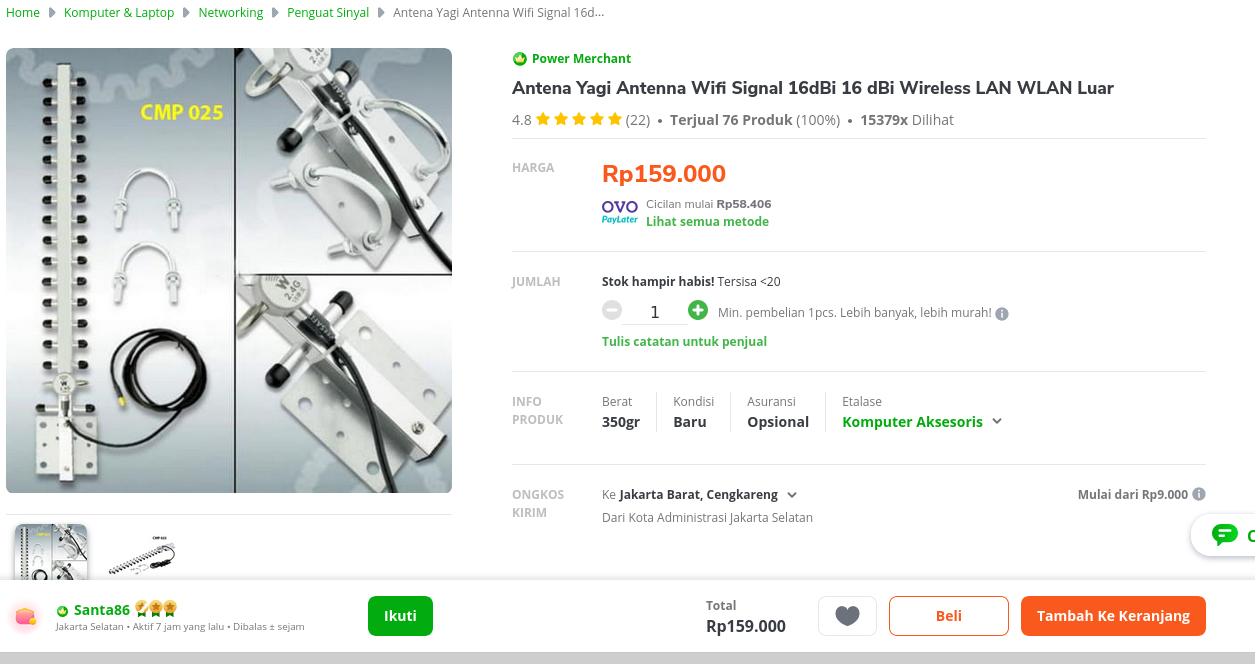
\includegraphics[scale=.3]{1a.png}
    \label{fig:antena_yagi}
    \caption{Antenna Yagi}
\end{minipage}
\begin{minipage}[!hbt]{\linewidth}
    \centering
    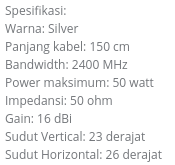
\includegraphics[scale=1]{1b.png}\\
    \label{fig:spesifikasi_yagi}
    \caption{Spesifikasi}
\end{minipage}
\newpage
Antenna Yagi tersebut memiliki panjang kabel 150cm.\\

\textbf{bandwidth 2400 Mhz}, atau setara dengan 2.4 Ghz. Berarti antena tersebut memiliki lebar frekuensi sebesar 2.4Ghz.\\

\textbf{Power maksimum 50watt}. Ketika antenna ini disambungkan ke transmitter, kekuatan tertinggi yang mampu ditangani oleh antenna ini tanpa
penurunan performa atau menimbulkan bahaya adalah 50 watt.\\

\textbf{Impedance 50 ohm}. Antenna ini di desain untuk transceivers dan kabel penghubung yang memiliki impedansi 50$\Omega$. Jika antena digunakan pada rangkaian
yang bukan 50$\Omega$ maka akan mengalami penurunan efisiensi pengiriman.\\

\textbf{Gain 16dBi}. Antenna ini memiliki kemampuan untuk memfokuskan energi yang dipancarkannya sebesar 16dBi, Semakin tinggi Gain, semakin fokus
energi yang dipancarkan.\\

\textbf{Sudut vertical $23^{\circ}$}. Artinnya sudut pancar vertikalnya adalah sebesar $23^{\circ}$.\\

\textbf{Sudut horizontal $26^{\circ}$}. Sudut pancar horizontalnya sebesar $26^{\circ}$.

\subsection{Antena Omni MIMO RNet WiFi 2.4Ghz + Pigtail + Packing}
\begin{minipage}{\linewidth}
    \centering
    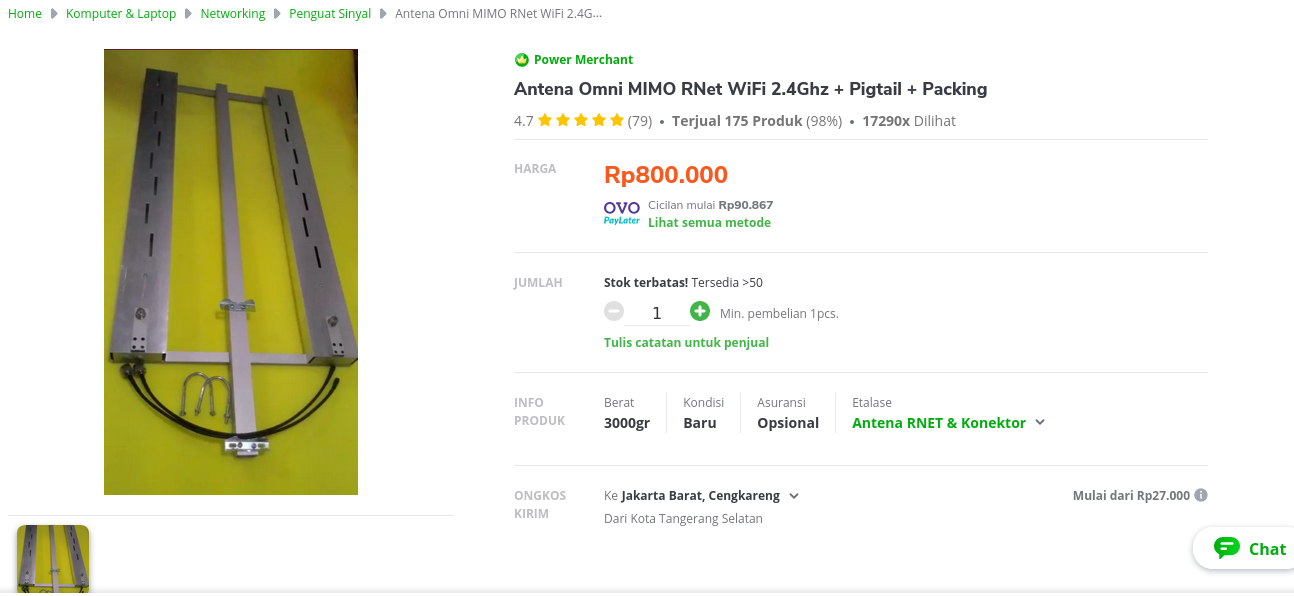
\includegraphics[scale=.3]{2a.png}
    \label{fig:antena_omni}
    \caption{Antenna Omni}
\end{minipage}
\begin{minipage}{\linewidth}
    \centering
    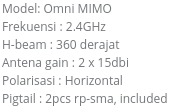
\includegraphics[scale=1]{2b.png}\\
    \label{fig:spesifikasi_omni}
    \caption{Spesifikasi}
\end{minipage}

\textbf{Model Omni}, Antena tersebut meradiasikan kurang lebih sama di sekitar antena dalam pola $360^{\circ}$.\\

\textbf{Frekuensi 2.4Ghz}, Antena memiliki jangkauan gelombang mikro. Pada Frekuensi 2.4Ghz panjang gelombangnya adalah
12.5 cm\\

\textbf{H-beam 360 derajat}, Sudut sebaran horizontal dari sinyal yang dipancarkan antena adalah $360^{\circ}$.

\textbf{Antena gain 2 $\times$ 15dbi}, Kemampuan untuk memfokuskan sinyal pada antena adalah sebesar 2 $\times$ 15dbi,
karena antena tersebut memiliki dua pemancar yang masing-masing memiliki gain sebesar 15dbi.

\textbf{Polarisasi horizontal}, Arah medan listrik yang diradiasikan berorientasi horizontal.

\subsection{Antenna Wifi Outdoor Grid Kenbotong TDJ-2400A 2.4GHz 24dBi}
\begin{minipage}{\linewidth}
    \centering
    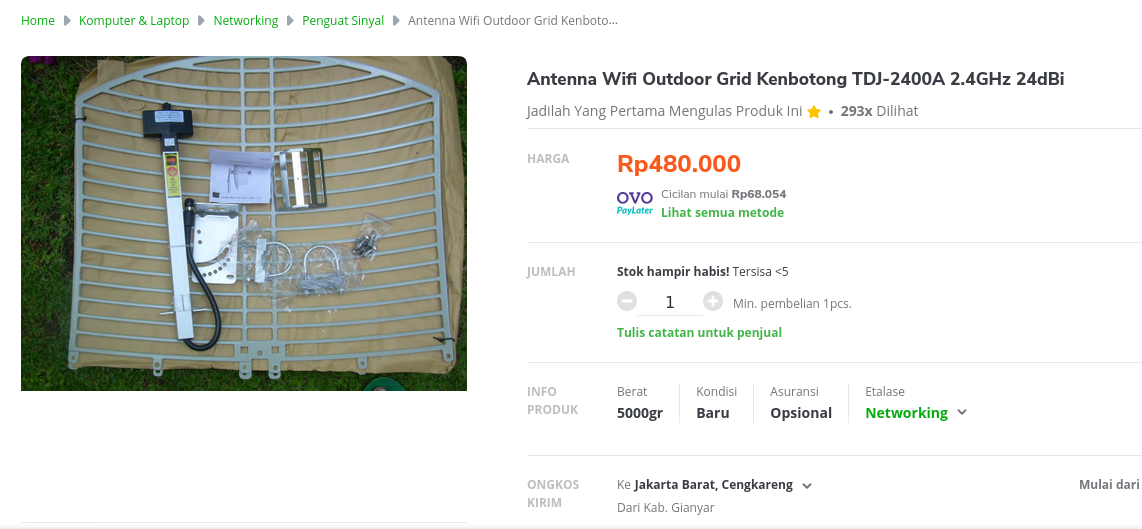
\includegraphics[scale=.3]{3a.png}\\
    \label{fig:antena_grid}
    \caption{Antena Grid}
\end{minipage}
\begin{minipage}{\linewidth}
    \centering
    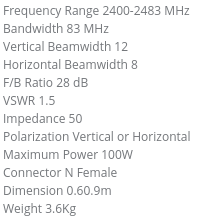
\includegraphics[scale=1]{3b.png}\\
    \label{fig:spesifikasi_grid}
    \caption{Spesifikasi}
\end{minipage}

\textbf{Frequency Range 2400-2483 MHz}, Antena memancarkan frekuensi dengan rentang 2400MHz-2483Mhz, yang termasuk dalam
golongan Ultra High Frequency (UHF).\\

\textbf{Bandwidth 83 MHz}Antena memiliki lebar frekuensi sebesar 83 MHz, Semakin besar bandwidth, maka semakin besar
pula satuan data yang dapat dikirimkan dalam satu waktu.\\

\textbf{Vertical Beamwidth 12} memiliki sudut pola vertikal antena sebesar 12 pada saat daya setengah.\\

\textbf{Horizontal Beamwidth 8} memiliki sudut pola horizontal antena sebesar 8 pada saat daya setengah.\\

\textbf{F/B Ratio 28 dB} Rasio penguatan maksimum pada arah antena terhadap arah yang berlawanan adalah sebesar 28dB\\

\textbf{VSWR 1.5} Antena memiliki kecocokan impedansi dengan saluran transmisi yang terhubung sebesar 1.5.\\

\textbf{Impedance 50} Antenna ini di desain untuk transceivers dan kabel penghubung yang memiliki impedansi 50$\Omega$. Jika antena digunakan pada rangkaian
yang bukan 50$\Omega$ maka akan mengalami penurunan efisiensi pengiriman.\\

\textbf{Polarization Vertical or Horizontal} Arah medan listrik yang diradiasikan bisa berorientasi vertikal atau
horizontal.

\textbf{Maximum Power 100W}, Ketika antenna ini disambungkan ke transmitter, kekuatan tertinggi yang mampu ditangani oleh antenna ini tanpa
penurunan performa atau menimbulkan bahaya adalah 100 watt.\\

\textbf{Connector N Female} Memiliki connector berjenis RF coaxial connector.

\end{document}
